\documentclass[10pt,twocolumn,letterpaper]{article}
\usepackage{cvpr}
\usepackage{times}
\usepackage{epsfig}
\usepackage{graphicx}
\usepackage{amsmath}
\usepackage{amssymb}
\usepackage{afterpage}

\newcommand\blankpage{%
    \null
    \thispagestyle{empty}%
    \addtocounter{page}{-1}%
    \newpage}

% Include other packages here, before hyperref.
% If you comment hyperref and then uncomment it, you should delete
% egpaper.aux before re-running latex.  (Or just hit 'q' on the first latex
% run, let it finish, and you should be clear).

\usepackage[pagebackref=true,breaklinks=true,letterpaper=true,colorlinks,bookmarks=false]{hyperref}

\cvprfinalcopy % *** Uncomment this line for the final submission

%\def\cvprPaperID{****} % *** Enter the CVPR Paper ID here
%\def\cvpr
\def\httilde{\mbox{\tt\raisebox{-.5ex}{\symbol{126}}}}

% Pages are numbered in submission mode, and unnumbered in camera-ready
\ifcvprfinal\pagestyle{empty}\fi
\begin{document}

%%%%%%%%% TITLE
\title{Speech Processing - Application of Probability}

%% Authors ---------------------------------------------------
\author{
Sreenya Chitluri\\
Roll No: 2020102065\\
{\tt\small sreenya.c@students.iiit.ac.in}

\and
Smruti Biswal\\
Roll No: 2020112011\\
{\tt\small smruti.biswal@research.iiit.ac.in}
\and
Akshit Gureja\\
Roll No: 2020112004\\
{\tt\small akshit.gureja@research.iiit.ac.in} 
}

\maketitle
\thispagestyle{empty}

%%%%%%%%%%%%%%%%%%%%%%%%%%%%%%%%%%%%%%%%%%%%%%%%%%%%%%%%%%%

%------ABSTRACT-------------------
\begin{abstract}
   Speech processing deals with the study of input speech signals and the methods of processing them. Speech processing involves several components in designing of speech systems, a lot of which use probability models. In this report, we will look into use of Gaussian random variables while modelling and filtering noise that gets added after being passed through an additive noise channel in a communication system, and, the applications of Hidden Markov's models in speech recognition. 
\end{abstract}

%%%%%%%%% Introduction %%%%%%%%%%%%%%%%%%%%%%%%%%%%%%%%%%%%%%%%
\section{\textbf{Introduction}}

Speech Processing is characterized by several components some of which being
\begin{enumerate}
    \item Speech Coding
    \item Speech Recognition
    \item Speech Enhancement, etc.
\end{enumerate}
The probability density function (pdf) of speech signals and noise should be well defined for an effective speech processing system. 
\vspace{0.35cm}
\par A major part of speech enhancement is the removal of noise that gets added through an additive noise channel. This is known as filtering and is a huge application of probability. An additive noise is a very important part of the communication systems and speech processing. They are based on Normal distribution and Gaussian Random Variables. As we remove noise, we can recognize speech better. This helps in efficiency in speech processing. 
\vspace{0.35cm}
\par Speech recognition involves enabling the identification and translation of the spoken language into text by computers. Hidden Markov Models are used as basis on modern speech processing units in general. The purpose of using Hidden Markov Models (HMMs) is because speech signal can be considered as short-time (or) piece-wise stationary signal i.e. it is assumed that statistical characteristics of the signal don't change with time. HMMs are statistical models whose output is a sequence of Random Variables (quantities or symbols). We assume that speech can be approximated to be a stationary process for a very short period of time, say 10 milliseconds. Thus speech is modelled as a Markov model for a stochastic process (or random processes). 
 HMMs are popular for another reason, this is because they can be 'trained' automatically and are simple and computationally viable in practical application. The HMM output sequence of of n-dimensional real valued vectors such that n is a small n. Each output is given output in 10 milliseconds. Thus Hidden Markov Models are important in Speech Recognition part of the speech processing.



%%%%%%%%%%%% Theoretic Preliminaries %%%%%%%%%%%%%%%%%%%%%%%%%%

\section{\textbf{Theoretic Preliminaries}}
For recognizing the importance of application of Random Variables and Random Processes we must be familiar with the concepts of Random Variables, Probability Density Function, Gaussian Random Variables, Central Limit Theorem, Additive Noise Channel and Stochastic processes. 

%--------------------------------------------------------------

\subsection{Random Variable}
A random variable, abbreviated as RV, is a variable whose values depends on the outcomes of a random phenomenon. If $X$ is a RV, then $$X: S \mapsto \mathbb{R}$$ such that $X$ is a measurable function. This means that it should be satisfying the following property:
 Pre-images are of the form $(-\infty, x]$, i.e., $X^{-1}((-\infty, x]) \in \mathcal{F}$ where $\mathcal{F}$ is the event space of the random phenomenon. 

%--------------------------------------------------------------

\subsection{Probability Density Function}
For a RV X with Cumulative Distribution Function (CDF) defined as $F_X(.)$ such that $$F_X(x) = P(X \leq x)$$

If $F_{X}(.)$ is continuous and say it has a differential, this differential is called as \textbf{Probability Density Function} (pdf) 
$$ f_{X}(x) = \frac{d}{dx}F_X(x)$$
Here, $f_{X}(x)$ is called as Probability density function. In probability, pdf of a continuous RV is a function whose value at any given sample is the set of possible values taken by the RV can be interpreted as providing a relative likelihood that the value of the random variable would equal that sample. Probability Density Function is used to specify the probability of the random variable falling within a particular range of values, as opposed to taking on any one value\\ 
Also,
$$ f_X(x) = \frac{d}{dx}F_X(x)$$
$$ \implies F_{X}(a) = P(X \leq a) = \int_{-\infty}^{a}f_{X}(x)dx$$
$$ P\left(a< X \leq b\right) = F_{X}(b) - F_{X}(a) = \int_{a}^{b}f_{X}(x)dx$$
If we plot $f_X(x)$ vs $x$ and consider the area between $x$ and $x+\Delta x$ We can also define
$P\left(x \leq X \leq x + \Delta x \right) \approx$ Area of rectangle with width $\Delta$ and height $f_{X}(x)$ provided $\Delta$ is very small
$$ P\left(a \leq X \leq b\right) = f_{X}(x) \Delta x $$
\textbf{Properties of pdf}
If a function has the following pdf then it is said to be a valid pdf of the given RV.
\begin{enumerate}
    \item $$f_X(x) \geq 0$$ i.e. $f_X(.)$ is monotonically non-decreasing function
    \item $$\int_{-\infty}^{\infty}f_X(x)dx = 1 $$ This is because $P(X<\infty)$ hence $F_X(\infty) = 1$
\end{enumerate}


%--------------------------------------------------------------


\subsection{Gaussian Random Variable}
A Gaussian RV is the RV used to describe a Gaussian distribution. The general form of the pdf of a Gaussian RV $X$ is: $$f_X(x) = \frac{1}{\sigma\sqrt{2\pi}}e^{-\frac{1}{2}(\frac{x-\mu}{\sigma})^2}$$ where $\mu$ is the mean, median and the mode of the distribution, and $\sigma^2$ is the variance. This RV has a lot of applications in modelling major aspects of signal processing, for eg, noise is represented as a Gaussian RV during speech processing.\\
\vspace{0.7cm}
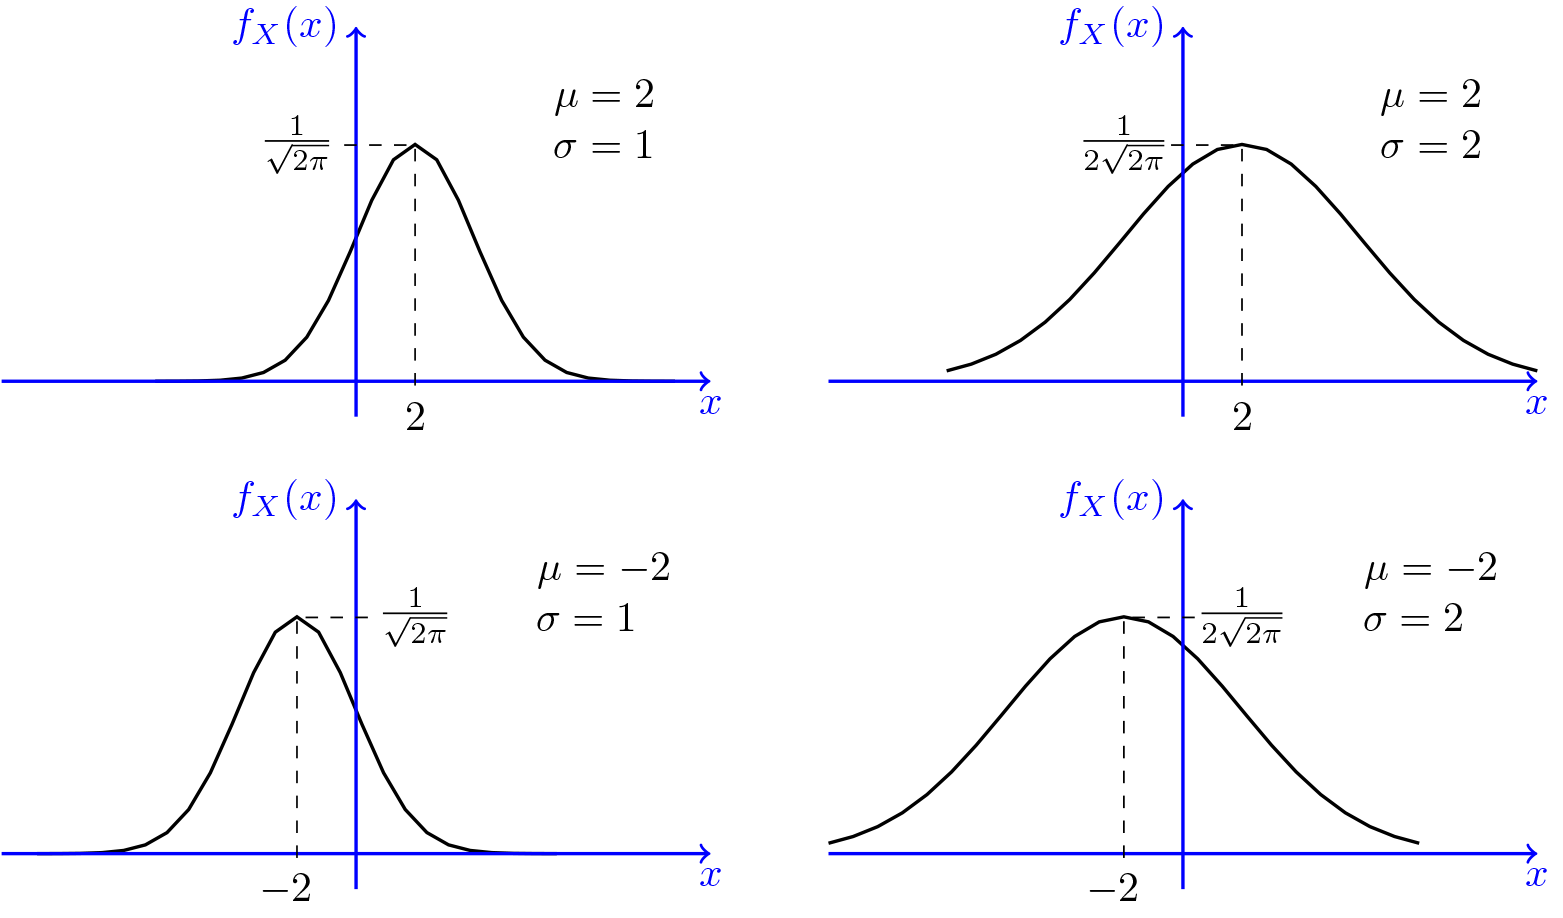
\includegraphics[scale=0.57]{gauss.png}
\begin{center}
    Fig 1: PDFs of example Gaussian RVs
\end{center}


%--------------------------------------------------------------


\subsection{Central Limit Theorem}
The central limit theorem states that when independent random variables are added, their properly normalized sum tends toward a normal (or Gaussian) distribution even if the original variables themselves are not normally distributed. The central limit theorem has several variants. Commonly, the random variables are independent and identically distributed (iid). In other forms, the convergence of the mean to the normal distribution also occurs for non-identical distributions, given they comply with certain conditions. \\
\textit{\textbf{Theorem:} $X_1,X_2,X_3 \dots X_n$ are a sequence of iid RVs where $E(X_i) = \mu$ and $Var(X_i)=\sigma ^2$ then}
$$ Z_n = \frac{\sum_{i=1}^{n}X_i - E\left(\sum_{i=1}^{n}X_i\right)}{\sqrt{Var(\sum_{i=1}^nX_i)}} $$
This is implied mostly when N is a large number. A simple example of the central limit theorem is rolling many identical, unbiased dice. The distribution of the sum (or average) of the rolled numbers will be well approximated by a normal distribution.

%--------------------------------------------------------------

\subsection{Additive Noise Channels}
Additive Noise Channels are of great importance in communication models. The channel input and the noises are both random processes. \textit{Random process is a mathematical object usually defined as a family of random variables.} Let the input signal be a random process $X(t)$ such that   
$$ \{X(t); t \in \mathbb{R}\}$$
And let the noise be $N(t)$ such that 
$$ \{N(t); t \in \mathbb{R}\}$$.
The channel output is another random process $Y(t)$ such that
$$ Y(t) = X(t) + N(t)$$
This means that if the time is fixed i.e. for a period of time \textbf{Random Variable} $Y$ is equal to \textit{sum of Random Variables} $X$ and $N$.
$$Y = X + N \hspace{0.2cm} given \hspace{0.1cm} t \hspace{0.1cm} is \hspace{0.1cm} fixed$$
We should note that noise in this channel can always be defines at the difference $Y(t) - X(t)$ between the output and the input signal. The notion of additive noise tells us that the processes are independent i.e. \textit{when time is constant the Random Variables formed are Independent in nature}. This nature of the channel incorporates that we know the following about the channel:
\begin{enumerate}
    \item channel attenuation
    \item propagation delay
    \item carrier frequency and phase
\end{enumerate}
It is also assumed that all noises are accommodated by the $N$ and the input speech signal is not distorted by any other factors.
Additive noise can be easily modelled by a Gaussian Random Variable and is frequently done as so. In other cases, when noise is not directly an Gaussian Random Variable, it is a modified version of Gaussian Random Variable. Most of the noise Random Variables, even though not explicitly mentioned as Gaussian Random Variables, are valid only for Gaussian Random variable and it's pdf.

%--------------------------------------------------------------

\subsection{Stochastic Process}
A stochastic process, in simple terms is a process that deals with probability and values changing with time. A stochastic process involves variables which change at random rate through time. And one of the simplest stochastic processes is a Markov Chain.





%%%%%%%%%%%%%%%%%%%%%% Applications %%%%%%%%%%%%%%%%%%%%%%%%%%%

\section{\textbf{Applications of Random Variables/Random Processes in Speech Processing}}

%--------------------------------------------------------------

\subsection{Speech Enhancement}
Speech enhancement aims to improve speech quality by using various methods. After speech passes through additive noise channel, we get disturbances which reduce the quality of speech for processing. So must remove the noise. Noise can be filtered easily if it modelled as a Random Variable (RV).

%--------------------------------------------------------------

\subsubsection{Modelling Noise as a RV}
Noise is often modelled as a Gaussian random variable. This is because noise is a by-product of a large number of independent small effects which can be represented as random variables. Applying central limit theorem, noise can be mathematically calculated to be a Gaussian random variable. The mean of this Gaussian random variable turns out to be 0.

\par Let $X_1, X_2, X_3, ...$ be independent random variables which contribute to noise. Using central limit theorem, we can define $$Z_n = \frac{\sum_{i=1}^nX_i-E(\sum_{i=1}^nX_i)}{\sqrt{Var(\sum_{i=1}^nX_i)}}$$
and say that the sequence $Z_1, Z_2, ...$ converges to $Z$ which is a Gaussian random variable with mean 0 and variance 1. Using this result, we can define the pdf of $Z$ as $$f_Z(z) = \frac{1}{\sqrt{2\pi}}e^{\frac{-z^2}{2}}$$ using pdf of Gaussian RV as defined before. Here, $Z$ is the noise that gets added to the speech signal after passing through an additive noise channel. As part of speech processing, we must filter out this noise. This is known as speech enhancement. 

%--------------------------------------------------------------

\subsubsection{Filtering of Noise}
Noise when modelled as a Gaussian RV has mean equal to 0 as described above. This is a crucial factor for the filtering of noise and getting better quality of speech signals. Let's say our input speech signal is a sinusoidal wave as described in Fig 1a. As it passes through an additive noise channel, noise gets added as shown in Fig 1b. \\

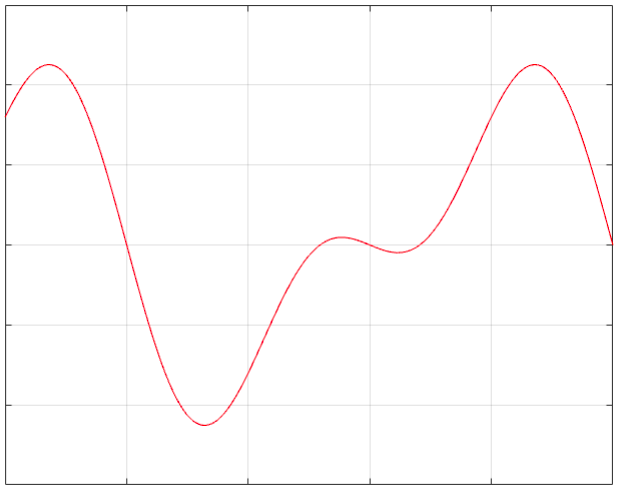
\includegraphics[scale=0.17]{original.png}
\hspace{0.4cm}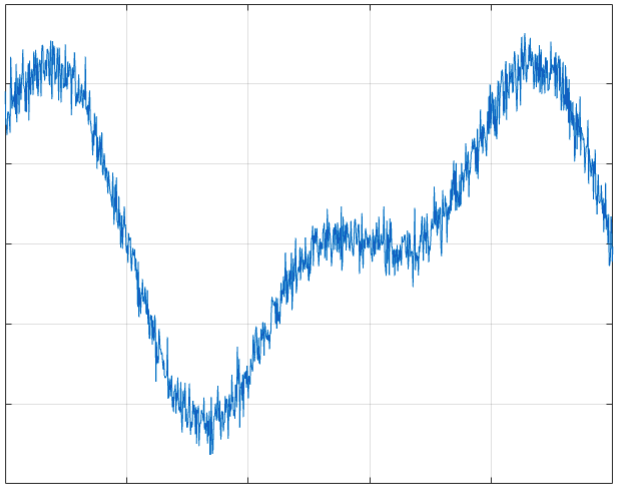
\includegraphics[scale=0.17]{noisy.png}
\begin{center}
    Fig 2a\hspace{3.5cm}Fig 2b   
\end{center}
The filter works by calculating the average of all the values of the signal from $a$ to $a+M$ and mapping it to the $(a+M+1)$\textsuperscript{th} point, where $a$ is any point in the signal domain and $M$ is a constant. We know that $$n = s + g$$ where $n, s, g$ are the noisy output signal, input speech signal and noise modelled as a Gaussian RV respectively. The filter takes input $n$ and gives an output signal which is expected to be the closest to $s$. Let this output signal be $o$. From the above analysis, we know that $$o_{a+M+1} = \frac{\sum_{i=a}^{a+M}n_i}{M}$$ Replacing $n$ with $s+g$, $$o_{a+M+1} = \frac{\sum_{i=a}^{a+M}(s_i+g_i)}{M} = \frac{\sum_{i=a}^{a+M}(s_i)+\sum_{i=a}^{a+M}(g_i)}{M}$$ As the value of $M$ increases, the term $\frac{\sum_{i=a}^{a+M}(g_i)}{M}$ tends to $E(g)$. As we modelled $g$ i.e. noise as a Gaussian RV with mean 0 and variance 1, $E(g)\to 0$ and $o_{a+M+1}\to \frac{\sum_{i=a}^{a+M}(s_i)}{M}$. We observe that as $M$ increases, $o$ becomes closer to $s$ but a shifted version of it as shown in Fig 2. This is known as an $M$-order filter. 
\begin{center}
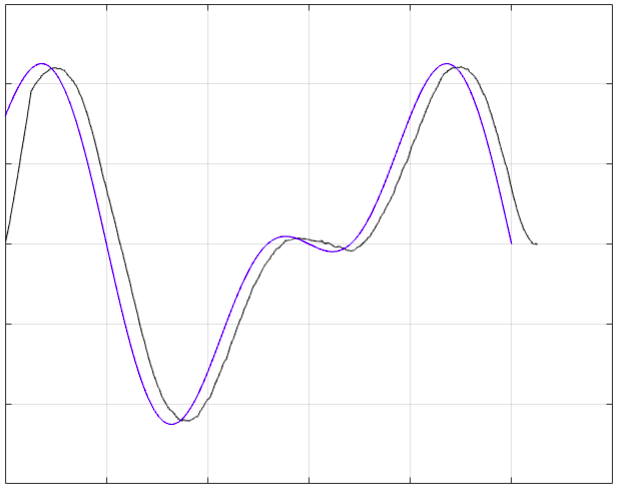
\includegraphics[scale=0.25]{orgvsfilt.png}\\
Fig 3: Filtered and original signals
\end{center}

So, by modelling noise as a Gaussian RV we can eliminate noises by using a simple filter as described above. And henceforth we improve the speech signal quality, hence enhancing it. This effective filter is called $M$-order filter.\\

%--------------------------------------------------------------
\subsection{Speech Recognition}

Now let's look at one more application of probability in the field of speech processing, which are Markov Chains and Hidden Markov Models.

%--------------------------------------------------------------

\subsubsection{Markov Chains}
A Markov Chain is a memory-less stochastic process, which means that the probability of future events is independent of any previous event till the present. This property of memory-less process is known as the \textbf{Markov Property}. \\

To explain in more clarity how Markov Chains differ from general Stochastic Processes, it would be good if we look at an example. \\

Suppose we have a bag of 5 Blue Balls, 3 Red Balls and 5 Green Balls, and we have to find the probability that the $3^{rd}$ ball we pick without replacement is Red in color. \\

Note that here, the probability that we are looking for depends on the number of Red balls left in the bag when we go for our $3^{rd}$ pick which is dependent on the balls that have been picked up in the first 2 picks. Thus, the probability that we aim to find depends on previous events and this is a general stochastic process.\\

Let's twitch the example a bit and now we are picking balls with replacements. So after each step, the number of balls in each color is independent of any picks we do at any step. This is analogous to a memory-less system in the sense that an future event is independent of any past probability or trial. This forms an example of a Markov Chain. \\

%--------------------------------------------------------------

\subsubsection{Directed Graph Representation}
One of the most common Markov chains are time-homogenous Markov Chains which are represented using directed graphs, like the one given below. In such cases, the probability of any state is independent of time.  
\begin{center}
    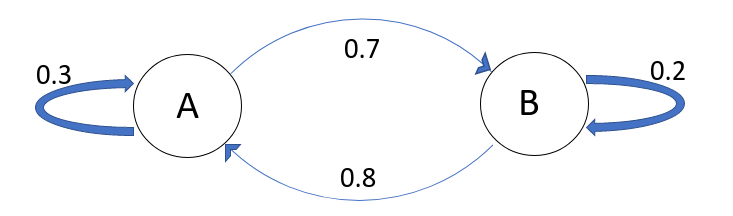
\includegraphics[scale=0.35]{Markov_Chain.png}
    Fig 4
\end{center}

In figure 4, each directed arrow is labelled which denotes the probability of going from one state to the one pointed to. So the probability of going from A to B is 0.7, and staying at A is 0.3. One important point to visualize is that the sum of the probabilities of all the arrows going out from a state must be 1 for a valid process. 

Suppose we are on ‘B’ as the starting point, and we need to move to A in 2 steps. 

This can be done, if in the first step we stay at B and move to A in 2nd step, the probability of which is 
\begin{center}
     = 0.2*0.8 = 0.16 
\end{center}

Another way is we move to A in the first step and stay at A during the 2nd, the probability corresponding to this is 
\begin{center}
    = 0.8*0.3 = 0.24
\end{center}
So, the total probability becomes 
\begin{center}
    0.16+0.24 = 0.4
\end{center}

A Markov Chain can then be assumed to be a sequence of random variables satisfying the rules of conditional independence. Thus, Markov Property can be stated formally as:- 

If $X_1, X_2 …. X_n$ are ‘n’ random variables and $a_1, a_2,... a_n$ depict the possible states. Then,
\begin{center}
    $P(X_n = a_n | X_{n-1} = a_{n-1}) = P(X_n = a_n | X_1 = a_1, X_2 = a_2, X_3 = a_3, …... X_{n-1} = a_{n-1}) $
\end{center}

In other words, knowledge of the previous states is all that is necessary to determine the probability distribution of the current state.  \\

\textbf{Note:} This doesn’t contradict our memory-less property, the probability of transitioning from one state to another is independent of any previous states we have been through. If we wish to get the probability distribution, we just need the knowledge of where we have been for analysis.

%______________________________________________________________

\subsubsection{Transition Matrix Representation}
A transition matrix $(P_t)$ for a Markov Chain at any time ‘t’ holds all the probabilities of transition between all possible states. The $(i,j)^{th}$ element of this matrix $P_t$ is given by: 
\begin{center}
    $(P_t)_{(i,j)} = P(X_{t+1} = j, X_{t = i})$ 
\end{center}

Thus each element of this matrix holds the conditional probability of moving from state ‘i’ which is the current position/ state of a random variable X at time ‘t’ to state ‘j’ in the next step. So, corresponding to our example in figure 4, the transition matrix can be given as -  

$$\begin{bmatrix}
0.3 & 0.7\\
0.8 & 0.2
\end{bmatrix}$$

%______________________________________________________________

\subsubsection{Hidden Markov Models}

Hidden Markov Model is a model which assumes that when a data of a system is being observed, what is being observed is not the state the system is in, but the data generated by some underlying hidden states. \\

For example, suppose we are listening to sound coming from a speaker. The sound which we listen to and is entering our ears is different from the state of the the speaker, which is the sound generating system. \\

In many real life applications, it is extremely difficult to predict the state of a system by just looking at the observations at hand. Hence, we use functions to map states to observations. Thus,
\begin{center}\begin{large}
    f(s) = o 
\end{large}
\end{center}
Where ‘s’ is used to denote the state of a system, which is mapped by the function ‘f(x)’ to an observation ‘o’. Thus, ‘o’ is the observation we make when function f(x) is applied to the state ‘s’ of a system.  \\

It is perfectly possible to have 2 different states $s_1, s_2$ being mapped to the same observation, in which case it forms a many-one function. Generally, in such cases, it is impossible to invert perfectly, because $f^{-1}(o)$ can be $s_1$ or $s_2$. \\

A Hidden Markov Model, is similar as when given an observation it can estimate the probability distribution over the possible states at any time, because many state sequences could lead to the same observation sequence. \\

In the field of Speech processing, the whole application of Hidden Markov Model in speech recognition revolves around the problem is estimating the system state (word spoken) behind the observations (sounds). \\

%______________________________________________________________

\subsubsection{Rules of Markov Models}
\begin{enumerate}
    \item \textbf{Markov Property : } \\
    The first rule is that the model must satisfy the Markov Property, according to which the model must be memory-less and the probability to transition from the current state to next depends only on the current state and independent of any past event or state the system as been through.
    
    $$P(s_t|s_{t-1}) = P(s_t|s_1,s_2,s_3....s_{t-1}) $$
    \item \textbf{Emit Observation After Each Transition} \\
    This rules for Markov Models states that after each transition from one state to another, the system must emit an observation dependent only on the current state. That is 
    
    $$P(o_{t}| s_{t})= P(o_t| s_t ,o_{t-1} ,s_{t-1} ,…,o_1 ,s_1 )$$
\end{enumerate}

Now, the observer gets to know only the observations and is unaware of the states and transitions that generated them; thus our hidden to the observer, giving the model its name – Hidden Markov Model(HMM). \\

An HMM is fully characterized by 5 parameters: 
\begin{enumerate}
    \item \textbf{Set of N states}\\
    $Q = s_1, s_2, s_3, .... s_N$
    \item \textbf{Set of T observations} \\
    $O = o_1, o_2, o_3,.... o_T$
    \item \textbf{Probabilities of State Transition}\\
    probability of transition from $s_i$ to $s_j$ denoted by $a_{i,j}$ and stored in the transition probability matrix A.
    \item \textbf{Conditional Observation Probabilities (Emission probabilities) } \\
    Probability that a model or system will emit an observation $o_t$ when in state $s_i$. That is $P(o_t | s_i)$ and is denoted by $b_{i}$. We take $B$ as the set of all these emission probabilities.
    \item \textbf{Probability of State Initialization:} \\
    The probability that the states of an HMM begin from the state $s_i$ and is denoted by $\pi_i$.
\end{enumerate}

We are now fairly equipped to study about the applications of Markov Chains and Hidden Markov Models in Speech Recognition. 

%______________________________________________________________

\subsubsection{Hidden Markov Models in Speech Recognition}
To move to Speech Recognition, we need to first understand phonemes.

%______________________________________________________________

\textbf{What are Phonemes?}
A phoneme is a unit of sound as small as 20 to 4 milliseconds, so it’s super super short. It is this unit which helps distinguish one word from another in a particular language. It is the tiniest part of the word, changing them changes the meaning of the word. Words like “thumb” and “dumb” are 2 different words and can be distinguished by just substituting one phoneme ‘th’ in thumb to ‘d’. \\

\textbf{Where do HMM's come here?}
Phoneme are put together in the correct sequence by using a Hidden Markov Model which does this ask by applying statistical probabilities. So we check how probable it is that one phoneme follows the first.  This can be put in 3 basic ideas or tasks.

\begin{enumerate}
    \item Represent speech as a sequence of observations that a system has made.
    \item Use HMM to model some unit of that speech, a word for example.
    \item Concatenate a single unit into larger units, phonemes to words and words to sentences for example.
\end{enumerate}

Lawrence Rabiner in 1989, characterized these as the 3 fundamental problems.
\begin{itemize}
    \item Problem 1 (Likelihood):\\ Given an HMM $\lambda$ and an observation Sequence O, find the likelihood $P(O|\lambda)$. 
    \item Problem 2 (Decoding) : \\
    Given Observation Sequence O and an HMM, estimate the best hidden state sequence Q, which maximizes probability of observation sequence 
    \item Problem 3 (Training) : \\
    Adjust parameters to maximize the probability of observed sequences.
\end{itemize}

We will look at the solutions to all these problems one by one.
\subsubsection{Likelihood Problem}
Often referred to as the Evaluation problem, we have the task to find $P(O|\lambda)$ when given the observation sequence $O = o_1, o_2, .... O_T$. 
Let's begin with a general approach to the task at hand.
We have an acoustic observation sequence $O = o_1, o_2... o_T$ and our goal is to estimate the word sequence spoken $W = w_1, w_2, .... w_M$. Let the estimated word be represented by $\hat{W}$. \\
\begin{align*}
    \hat{W} &= argmax \frac{P(O|W)P(W)}{P(O)} \\
    \hat{W} &= argmax P(O|W)P(W)
\end{align*}

However, this leads the give an exponential time complexity of $O(N^T)$, N being the possible states which can be reached. This is not favourable to be used in real life as it makes the computations slow, and increasingly time-consuming. \\

For which we use algorithms based on Dynamic Programming called as Forward Procedure. This algorithm uses a variable
$\alpha_t(i)$ representing the probability to be in state $i$ after seeing the $t-length$ observation sequence $o_1, o_2,... o_t$. Each probability $\alpha_t(i)$ is computed by summing the probabilities over paths that lead to the current state, and this lends to the algorithm it's recursive nature which greatly reduces the time complexity. 
Thus the whole algorithm can be summarized in 3 steps: \\
\begin{align*}
    &Initialization = \alpha_t(i) = \pi_i.b_i(o_i) & i \epsilon [1, N]\\
    &Recursion = \alpha_{t+1}(j) = \sum_{i=1}^{N}\alpha_t(i)a_{i,j}b_j(o_{t+1})&t \epsilon [1, T-1], j \epsilon [1, N] \\
    &Termination = P(O|\lambda) = \sum_{j=1}^{N}\alpha_T(j)\\
\end{align*}

\subsubsection{Decoding Problem}
The algorithm we use for decoding is the Viterbi algorithm. Using this algorithm we consider only the optimal decoding sequence corresponding to maximum likelihood and not all potential paths. This algorithm is also based on dynamic programming like the forward procedure used in the previous step. \\

This algorithm uses a variable $v_t(i)$ which represents the probability of being in state $i$ after looking at the $t$ observations and going through most probably state sequence $s_1, s_2,... s_{t-1}$. Thus,
\begin{align*}
    v_t(i) = \mathop{max}_{s_1, s_2,....s_{t-1}}( P(s_1, o_1, s_2, o_2,... s_{t-1}, o_{t-1}, o_t))
\end{align*}

Similar to the forward procedure, here we compute the Viterbi probability by getting the highest probability states which lead to the current state of the system. This lends to the decoding it's recursive nature and we can say- \\
\begin{align*}
    v_t(i) = \mathop{max}_{i = 1 to N} (v_{t-1}(i)a_{i,j}b_j(o_t))
\end{align*}

\subsubsection{Training and Learning Problem}
This is the toughest part of the process which is done using the Baum-Welch Algorithm. This algorithm helps the system learn about the transition probabilities and the probabilities of emission of the observation. It gives the model the flexibility to adjust the parameters to get the best Hidden Markov Model for a given sequence.

The algorithm works on the idea that if we know the probability distribution of the states at the time 't', we can get the transition and emission probability. However, more detail into the algorithm goes beyond the scope of our report.

This sums up the application of Markov Models in the speech recognition systems. In most of the modern day state-of-the-art systems used in speech and audio recognition a hybrid of HMM's and Neural Networks is used to deliver the best performance.

%%%%%%%%% Results and Conclusion %%%%%%%%%%%%%%%%%%%%%%%%%%%%%%
\section{Results and Discussion}

\begin{center}
    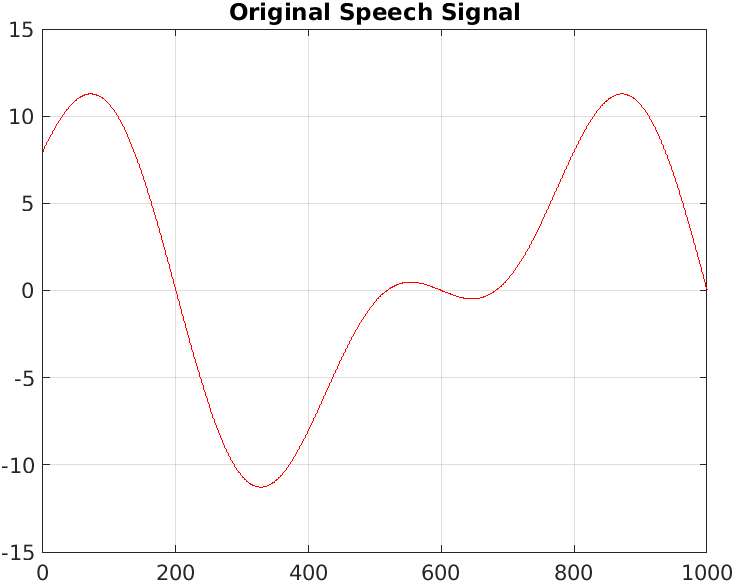
\includegraphics[scale=0.55]{Original.png}\\
    This is the original speech signal before it passes through any noisy channel. 
\end{center}

\begin{center}
    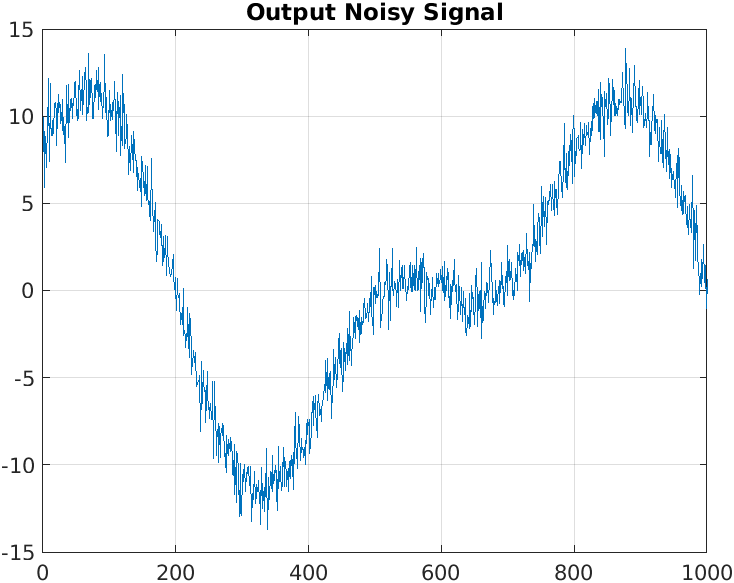
\includegraphics[scale=0.55]{NoisyOutput.png}\\
    After being passed through an additive noise channel, the signal appears to look like this. The noise added is normally distributed and can be modelled as a Gaussian RV with mean 0 and variance 1. 
\end{center} \vskip 0.2cm

\begin{center}
    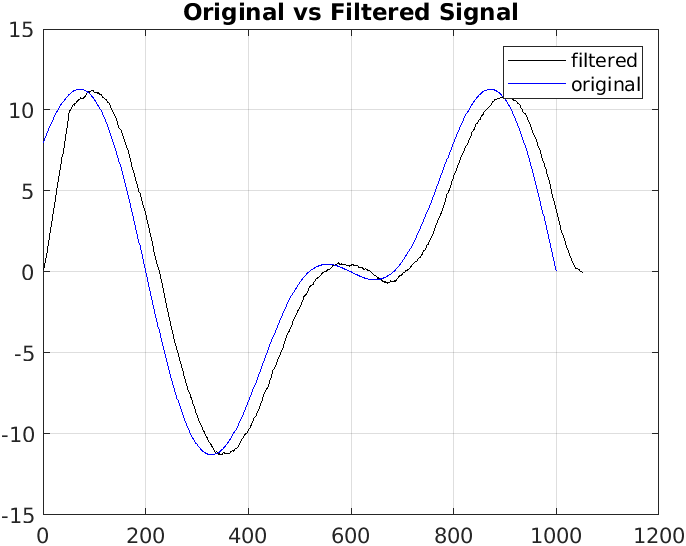
\includegraphics[scale=0.6]{OrginalvsFiltered.png}\\
    Taking into advantage that the mean of the noise is 0, the output of the $M$-order filter with $M=51$ resembles the original signal but it is shifted right. 
\end{center} \vskip 0.2cm

\begin{center}
    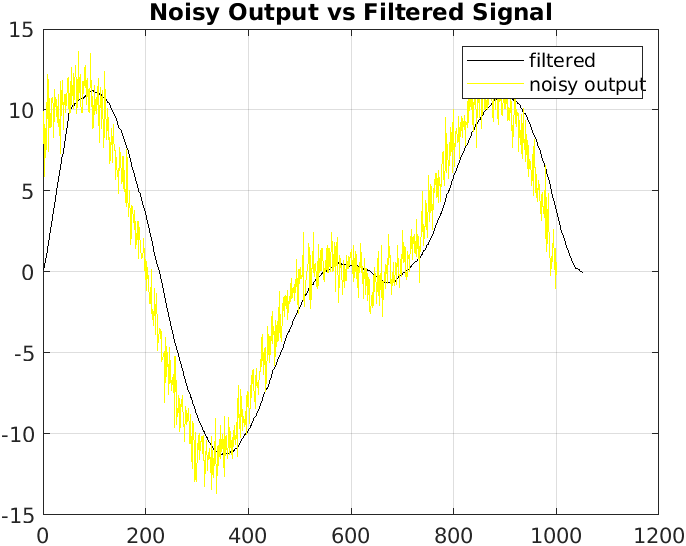
\includegraphics[scale=0.6]{noisyvsfilt.png}\\
    This is the output of the $M$-order filter vs the output of the additive noise channel.
\end{center}

\begin{center}
    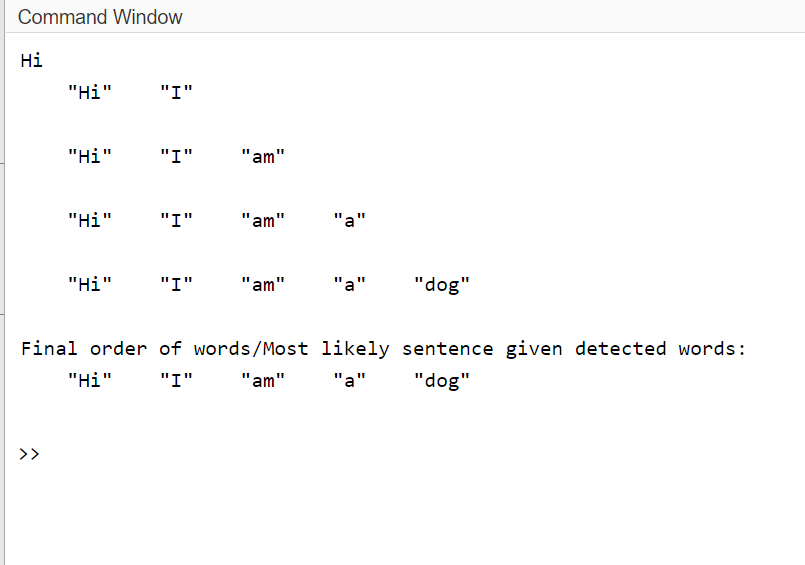
\includegraphics[scale=0.6]{MarkovOutput.png}\\
    Given the detected set of words, using Markov's model of speech recognition, we can predict the center.
\end{center}









\section{Conclusion}

\par Therefore, we have identified many crucial applications of probability in speech processing. Initially we started with Speech Enhancement which included filtering of signal as it comes out of additive noise channel. We applied the concepts of Gaussian Random Variables, Central Limit Theorem and Random Processes at constant time. We related the input, noise and output of a additive noise channel as Random Processes, then when we view them under constant time they can be considered as Random Variables. Noise , as we know, is a result of several independent Random Processes, and hence Central Limit Theorem is used to model Noise as a Gaussian RV with mean $\mu$ tending to 0. Taking this fact as an advantage, we design an filter which produces the outputs by taking the average value of certain points such that the Gaussian Noise is removed. This filter is simple yet efficient. This is called an $M$-order filter. \\

\par We have also been introduced to the concepts of Markov Chains, Hidden Markov Models and their applications in the field of speech processing and speech recognition. We started from the basics of Markov Chains and built ideas on top of them. We applied our knowledge of Markov Chains and Stochastic Processes to get more complex Models like the Hidden Markov Models which relate a sequence of states to the observations seen and help us determine the hidden states the system would have passed through. This process was distributed into three fundamental problems of Likelihood, Decoding and Training and we studied in brief how the Forward procedure, Viterbi, Baum-Welch algorithms give solutions to these problems.


%%%%%%%%% References %%%%%%%%%%%%%%%%%%%%%%%%%%%%%%%%%%%%%%%%%%
\section{References}
\begin{enumerate}
    \item 
    \url{https://ocw.mit.edu/courses/electrical-engineering-and-computer-science/6-450-principles-of-digital-communications-i-fall-2006/lecture-notes/book_7.pdf}
    \item 
    \url{https://web.sonoma.edu/users/f/farahman/sonoma/courses/ces540/lectures/Chapter6_Dig_Random_Proc.pdf}
    \item \url{https://en.wikipedia.org/wiki/Speech_enhancement}
    \item \url{https://en.wikipedia.org/wiki/Central_limit_theorem#Applications_and_examples}
    \item \url{https://en.wikipedia.org/wiki/Probability_density_function}
    \item \url{https://brilliant.org/wiki/hidden-markov-models/}
    \item \url{https://brilliant.org/wiki/markov-chains/}
    \item \url{https://www.cse.iitb.ac.in/~nirav06/i/HMM_Report.pdf}
    \item \url{https://web.stanford.edu/~jurafsky/slp3/A.pdf}
    \item \url{https://towardsdatascience.com/markov-chains-and-hmms-ceaf2c854788}
    \item \url{https://towardsdatascience.com/markov-and-hidden-markov-model-3eec42298d75}
    \item \url{https://jonathan-hui.medium.com/speech-recognition-gmm-hmm-8bb5eff8b196}
    
\end{enumerate}
\newpage
\pagebreak
\afterpage{\blankpage}
\afterpage{\blankpage}
\textbf{\Large Link To GitHub Repository:}\\
\url{https://github.com/AkshitGureja/PNRP-Project-Team-17.git}\\
\newline
\textbf{\Large Contributions:}
\begin{itemize}

\newline
\item\large Sreenya Chitluri
\begin{enumerate}
    \item Theoretic Preliminaries
    \item Speech Enhancement
    \item Introduction, Results 
    \item Coding: M-order filter, Markov Chains - I
\end{enumerate}
\item\large Smruti Biswal
\begin{enumerate}
    \item Theoretic Preliminaries
    \item Speech Enhancement
    \item Introduction, Results
    \item Coding: Gaussian noise, Markov Chains - II
\end{enumerate}
\item\large Akshit Gureja
\begin{enumerate}
    \item Theoretic Preliminaries
    \item Speech Recognition 
    \item Results
    \item Coding: Markov Chains - III
\end{enumerate}
\end{itemize}
\end{document}